\documentclass[a4paper, 11pt]{article}

\usepackage{a4wide}
\usepackage{graphicx}
\usepackage[utf8]{inputenc}

\title{Flixster data}
\author{Raphaël Fournier-S'niehotta, Tiphaine Viard}
\date{}

\begin{document}
	\maketitle
	
	Links graph $L =( V_L, E_L)$ : social network between users
	\begin{itemize}
		\item $|V_L|=786936$,
		\item $|E_L|=5897324$,
		\item $\delta(L)=1.9\cdot 10^{-5}$. %0.000019046128464401992.
		\item Une composante connexe géante
	\end{itemize}
	
	Bipartite ratings graph $R =( \top_R, \bot_R, E_R)$ : ratings of movies by users
	\begin{itemize}
		\item $|\top_R|=147612$ (users),
		\item $|\bot_R|=48794$ (movies),
		\item $|E_R|=8196065$,
		\item $\delta(R)=2.2\cdot 10^{-3}$,
		\item Une composante connexe géante.
	\end{itemize}
	
	\noindent
	Number of users in social network : 786936\\
	Number of users in ratings : 147612\\
	Number of users in friends but not ratings $|V_L \cap \top_L|$ : 147335\\
	%Number of users in ratings but not friends : 147335\\
	
	
	
	\begin{figure}
		\centering
		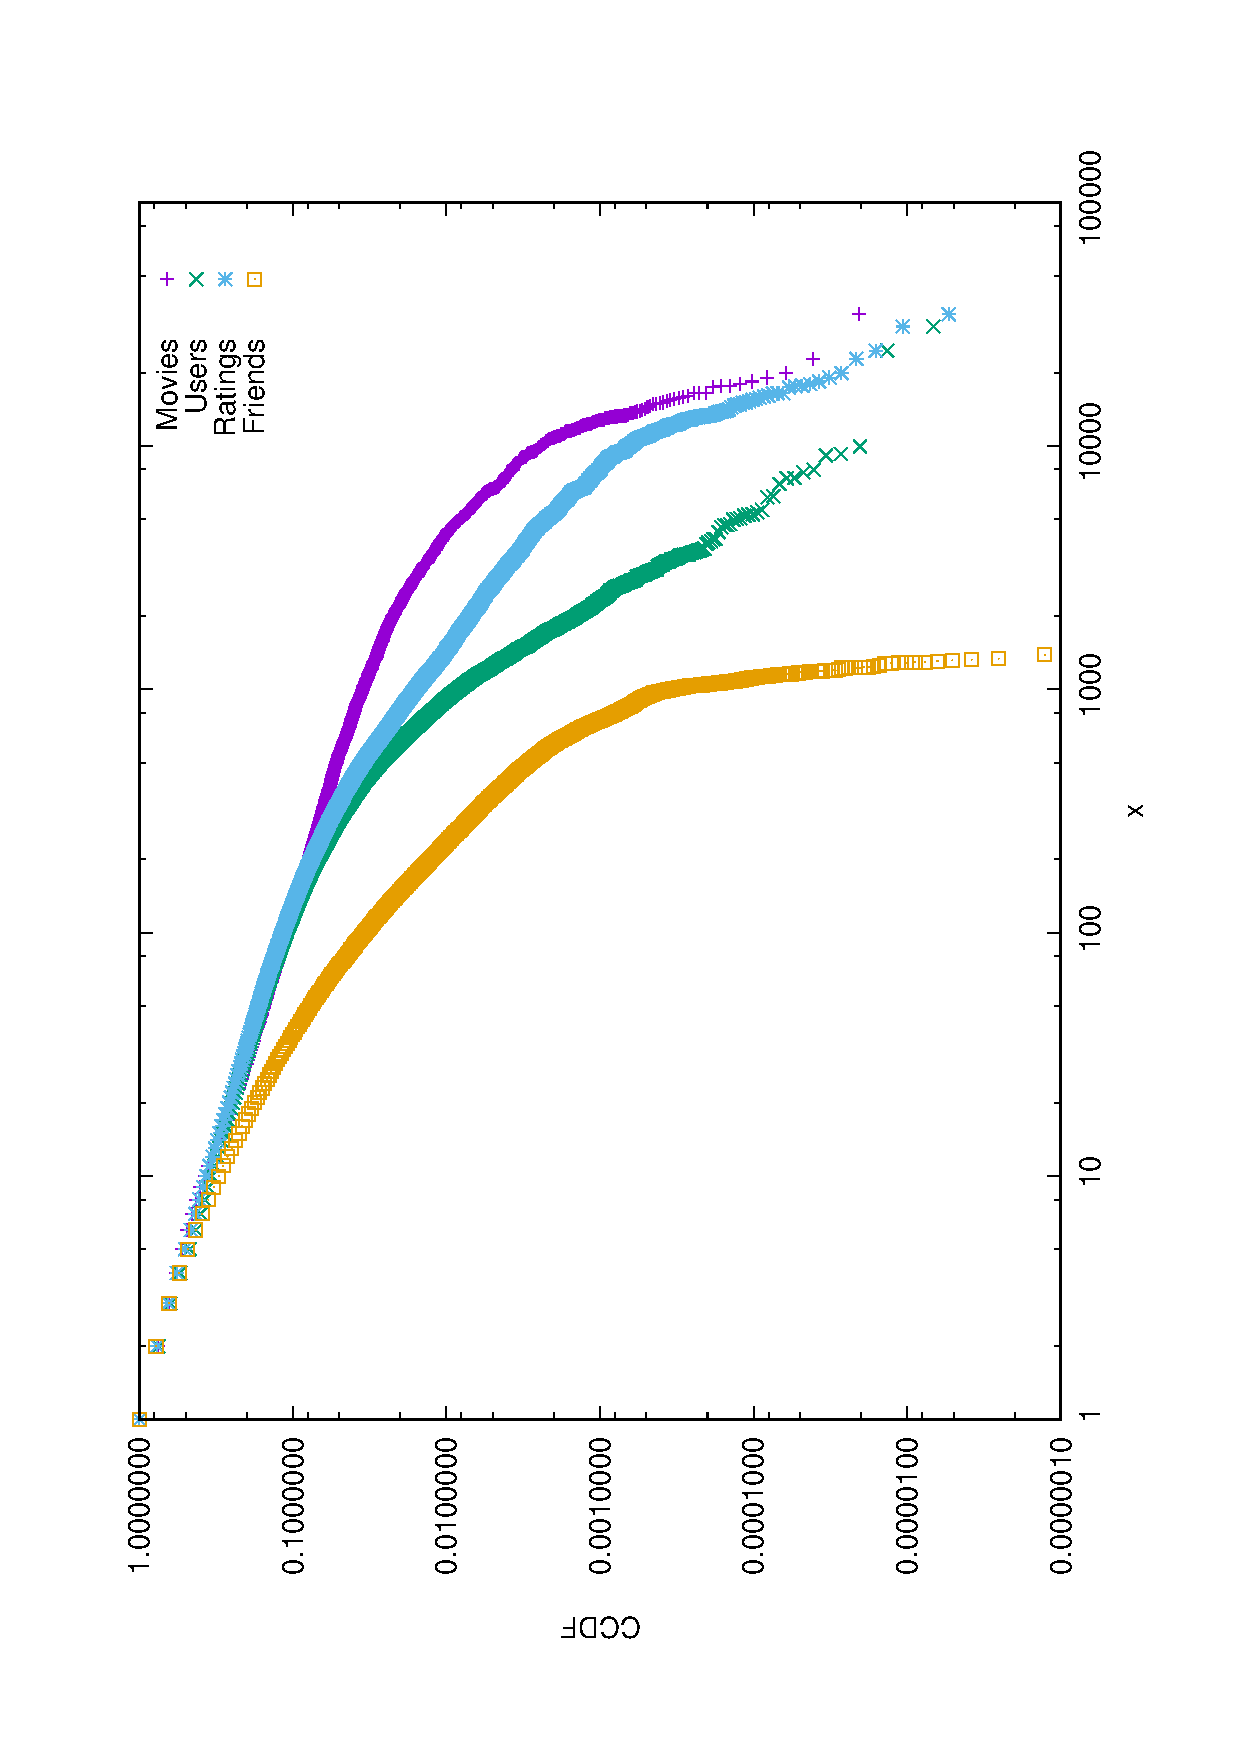
\includegraphics[angle=-90, width=0.9\linewidth]{img/ccdfs}
		\label{fig:degrees-ccdfs}
		\caption{Inverse cumulative degree distributions.}
	\end{figure}
	
	\begin{figure}
		\centering
		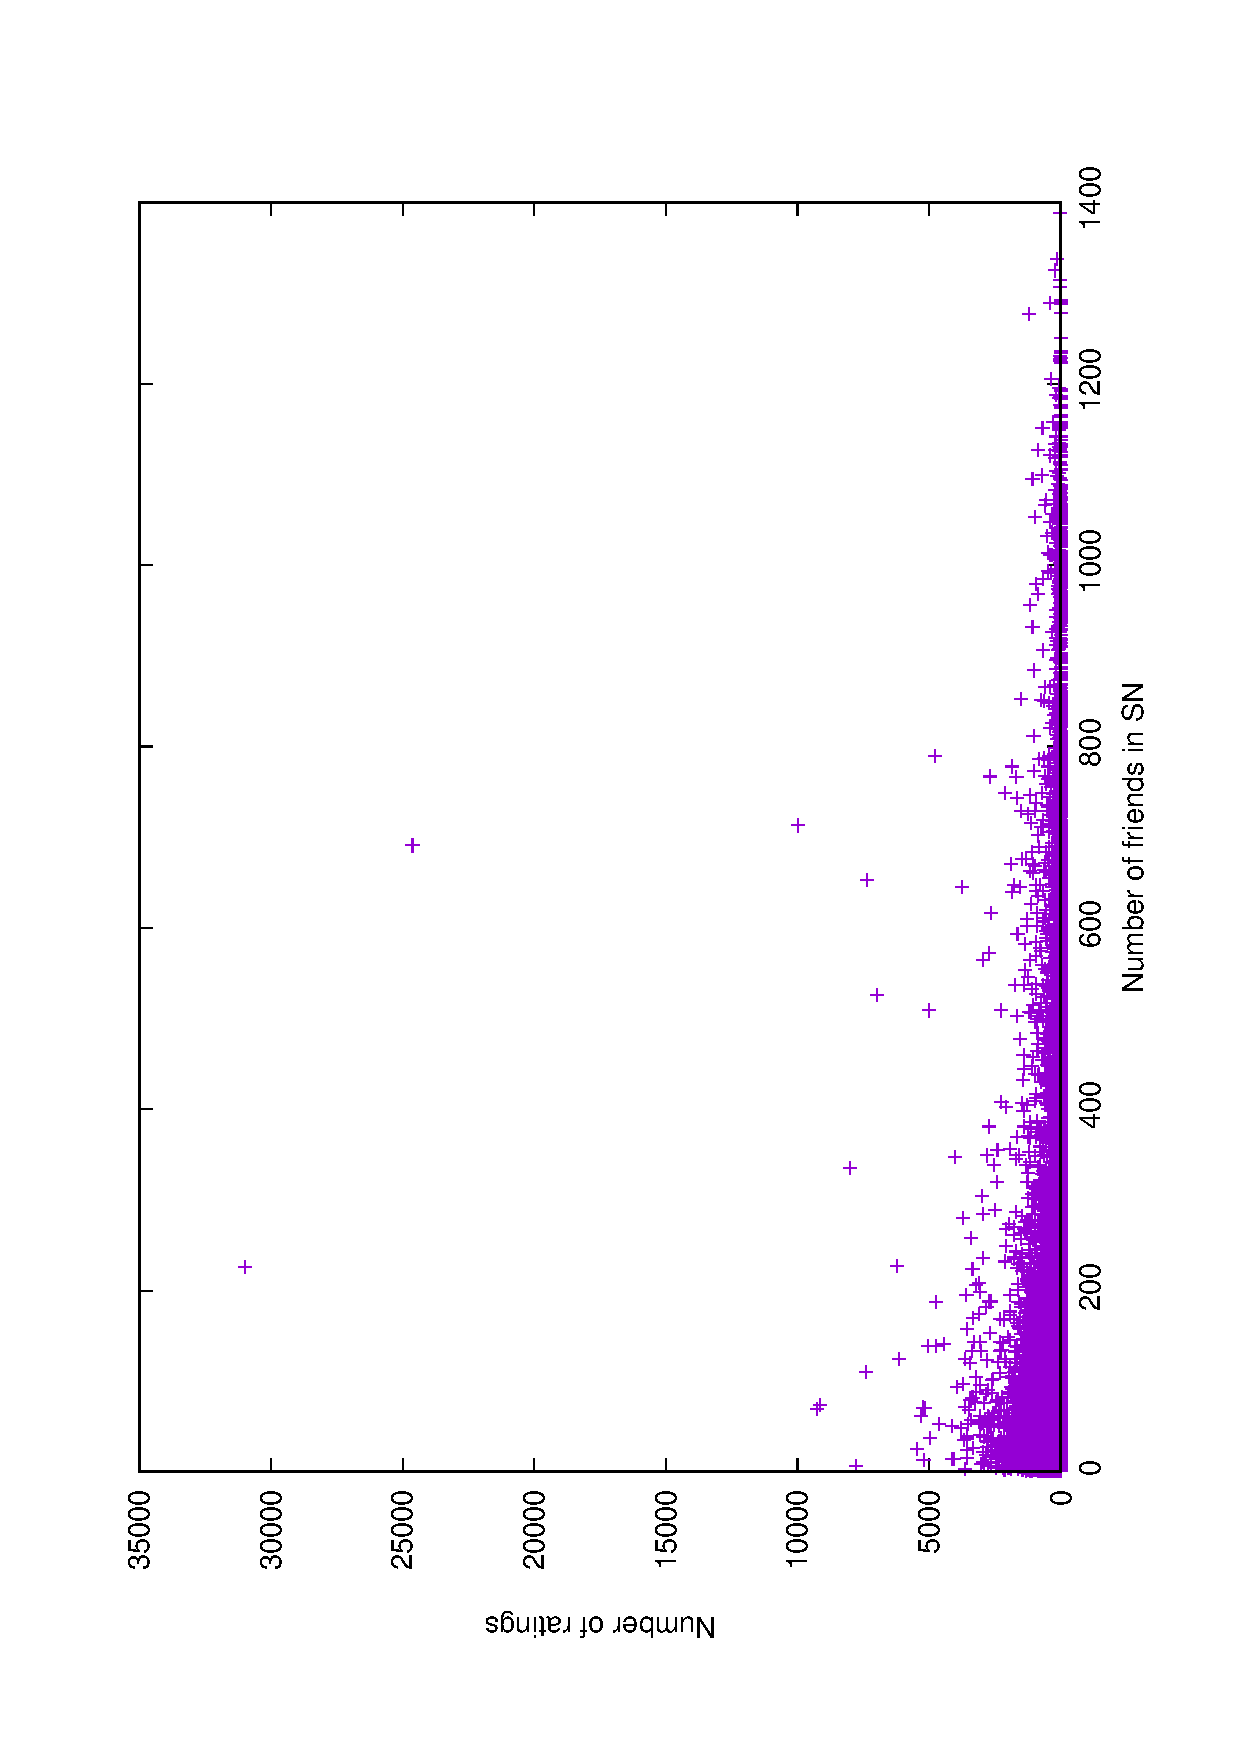
\includegraphics[angle=-90, width=0.9\linewidth]{img/degree-sn-vs-ratings}
		\label{fig:degrees-ccdfs}
		\caption{Inverse cumulative degree distributions.}
	\end{figure}
	
	
	En retirant les n\oe uds qui n'ont aucun rating, il reste $137925$ n\oe uds; Il y a environ 10000 n\oe uds qui ont des ratings mais sont connectés à des n\oe uds qui n'ont aucun rating.
	
	\clearpage
	
	\section{Prédiction de liens}

	Peut-on prédire les liens du réseau social en utilisant des méthodes de prédiction de liens sur le biparti (voir figure~\ref{fig:linkpred-bip-rs}).
	
	\begin{figure}
		\begin{center}
			\includegraphics[width=0.5\linewidth]{img/linkpred-bip-rs}
			\label{fig:linkpred-bip-rs}
			\caption{}
		\end{center}
	\end{figure}
	
	Ou alors, peut-on faire de la prédiction de liens sur le biparti en pondérant par l'existence ou non d'un lien dans le réseau social, voir figure~\ref{fig:linkpred-bip-rs} ?
	
	On cherche à prédire la note que $u$ donnerait à $F$, $\hat{S}_F(u)$.
	
	$$
		\hat{S}_F(u) = \sum_{v\in N(F)} \alpha_{uv}\cdot \beta_{uv} \cdot S_F(v)
	$$
	
	où $S_F(v)$ est la note donnée par $v$ pour le film $F$, $N(F)$ est le voisinage du film $F$,
	
	$$
		\alpha_{uv} = 1\mathtt{ si }\exists (u,v)\in E_L, [0,1] \mathtt{ si ... ?,} 0\mathtt{ (?) sinon.}
	$$
	
	et
	
	$$
	\beta_{u,v} = \mathtt{Jaccard ?}
	$$.
	
	
	Quelles sont les conditions limites ? On veut peut-être plutôt $argmax(\alpha_{uv}\cdot\beta_{uv})$, pour éviter de recommander des films très mal notés par $v$ ? On peut voir $\alpha_{uv}\cdot\beta_{uv}$ comme un terme de confiance de la recommandation.
	
	
	\section{Étude du projeté}
	
	Idée : comparer le projeté du biparti sur les utilisateurs au réseau social entre utilisateurs. 
	
	Dans la littérature, le projeté est souvent pondéré (par ex par le degré du n\oe{}ud projetant, le Jaccard entre les n\oe{}uds, etc.). Empiriquement, pondérer avec Jaccard donne de meilleurs résultats pour la détection de communautés.
	
	Tiph : j'ai un souci; on peut en discuter, mais je n'arrive pas à coder le projeté correctement : soit je stocke le projeté en RAM (et ça explose), soit je fais quelque chose qui ne stocke rien, mais là ça prend beaucoup trop de temps ... C'est comme tu imagines les n\oe{}uds de grand degré qui sont bloquants (pour nous ça tourne autour de 30 000 voisins, voir la distribution des degrés dans ce document).
	
	On pourrait mettre un seuil pour le projeté, mais ça me paraît très hasardeux, s'il n'y a pas de méthode "classique" dans la littérature pour le faire ?
	
	
	
\end{document}